\documentclass[11pt,utf8,notheorems,compress,t]{beamer}
\usepackage{etex}

\usepackage{pgfpages}
\setbeameroption{show notes on second screen}
\setbeamertemplate{note page}[plain]
\newcommand{\jnote}[2]{\only<#1>{\note{\justifying#2\par}}}

% Workaround for the issue described at
% https://tex.stackexchange.com/questions/164406/beamer-using-href-in-notes.
\newcommand{\fixedhref}[2]{\makebox[0pt][l]{\hspace*{\paperwidth}\href{#1}{#2}}\href{#1}{#2}}

\usepackage[english]{babel}

\usepackage{mathtools}
\usepackage{booktabs}
\usepackage{stmaryrd}
\usepackage{array}
\usepackage{ragged2e}
\usepackage{multicol}
\usepackage{tabto}
\usepackage{xstring}
\usepackage{ifthen}
\usepackage{soul}\setul{0.3ex}{}
\usepackage[all]{xy}
\xyoption{rotate}
\usepackage{tikz}
\usetikzlibrary{calc,shapes,shapes.callouts,shapes.arrows,patterns,fit,backgrounds,decorations.pathmorphing}
\hypersetup{colorlinks=true}

\graphicspath{{images/}}

\usepackage[protrusion=true,expansion=true]{microtype}

\setlength\parskip{\medskipamount}
\setlength\parindent{0pt}

\title{How topos theory can help commutative algebra}
\author{Ingo Blechschmidt}
\date{June 29th, 2018}

\useinnertheme[shadow=true]{rounded}
\useoutertheme[subsection=false]{miniframes}
\setbeamerfont{block title}{size={}}

\useinnertheme{rectangles}

\usecolortheme{orchid}
\usecolortheme{seahorse}
\definecolor{mypurple}{RGB}{150,0,255}
\setbeamercolor{structure}{fg=mypurple}
\definecolor{myred}{RGB}{150,0,0}
\setbeamercolor*{title}{bg=myred,fg=white}
\setbeamercolor*{titlelike}{bg=myred,fg=white}
\setbeamercolor{frame}{bg=black}

\usefonttheme{serif}
\usepackage[T1]{fontenc}
\usepackage{libertine}

\newcommand{\A}{\mathcal{A}}
\newcommand{\B}{\mathcal{B}}
\renewcommand{\AA}{\mathbb{A}}
\renewcommand{\C}{\mathcal{C}}
\newcommand{\E}{\mathcal{E}}
\newcommand{\F}{\mathcal{F}}
\newcommand{\M}{\mathcal{M}}
\renewcommand{\G}{\mathcal{G}}
\newcommand{\J}{\mathcal{J}}
\newcommand{\GG}{\mathbb{G}}
\renewcommand{\O}{\mathcal{O}}
\newcommand{\K}{\mathcal{K}}
\newcommand{\NN}{\mathbb{N}}
\newcommand{\QQ}{\mathbb{Q}}
\newcommand{\RR}{\mathbb{R}}
\newcommand{\TT}{\mathbb{T}}
\newcommand{\PP}{\mathbb{P}}
\newcommand{\ZZ}{\mathbb{Z}}
\renewcommand{\P}{\mathcal{P}}
\newcommand{\aaa}{\mathfrak{a}}
\newcommand{\fff}{\mathfrak{f}}
\newcommand{\ppp}{\mathfrak{p}}
\newcommand{\mmm}{\mathfrak{m}}
\newcommand{\defeq}{\vcentcolon=}
\newcommand{\defeqv}{\vcentcolon\equiv}
\newcommand{\Sh}{\mathrm{Sh}}
\newcommand{\GL}{\mathrm{GL}}
\newcommand{\Zar}{\mathrm{Zar}}
\newcommand{\op}{\mathrm{op}}
\newcommand{\Set}{\mathrm{Set}}
\newcommand{\Ring}{\mathrm{Ring}}
\newcommand{\LocRing}{\mathrm{LocRing}}
\newcommand{\Eff}{\mathrm{Ef{}f}}
\newcommand{\Sch}{\mathrm{Sch}}
\newcommand{\Aff}{\mathrm{Aff}}
\newcommand{\LRS}{\mathrm{LRS}}
\newcommand{\Hom}{\mathrm{Hom}}
\newcommand{\Spec}{\mathrm{Spec}}
\newcommand{\lra}{\longrightarrow}
\newcommand{\RelSpec}{\operatorname{Spec}}
\renewcommand{\_}{\mathpunct{.}}
\newcommand{\?}{\,{:}\,}
\newcommand{\speak}[1]{\ulcorner\text{\textnormal{#1}}\urcorner}
\newcommand{\ull}[1]{\underline{#1}}
\newcommand{\affl}{\ensuremath{{\ull{\AA}^1}}}
\newcommand{\Ll}{\text{iff}}
\newcommand{\inv}{inv.\@}
\newcommand{\seq}{\vdash_{\!\!\!\vec x}}
\newcommand{\hg}{\mathbin{:}}  % homogeneous coordinates

\setbeamertemplate{blocks}[rounded][shadow=false]

% Adapted from https://latex.org/forum/viewtopic.php?t=2251 (Stefan Kottwitz)
\newenvironment<>{hilblock}{
  \begin{center}
    \begin{minipage}{9.05cm}
      \setlength{\textwidth}{9.05cm}
      \begin{actionenv}#1
        \def\insertblocktitle{}
        \par
        \usebeamertemplate{block begin}}{
        \par
        \usebeamertemplate{block end}
      \end{actionenv}
    \end{minipage}
  \end{center}}

\newcommand{\bignumber}[1]{
  \renewcommand{\insertenumlabel}{#1}\scalebox{1.5}{\usebeamertemplate{enumerate item}}
}

\newenvironment{indentblock}{%
  \list{}{\leftmargin\leftmargin}%
  \item\relax
}{%
  \endlist
}

\newcommand{\hcancel}[5]{%
  \tikz[baseline=(tocancel.base)]{
    \node[inner sep=0pt,outer sep=0pt] (tocancel) {#1};
    \draw[red, line width=0.4mm] ($(tocancel.south west)+(#2,#3)$) -- ($(tocancel.north east)+(#4,#5)$);
  }%
}

\tikzset{
  invisible/.style={opacity=0,text opacity=0},
  visible on/.style={alt={#1{}{invisible}}},
  alt/.code args={<#1>#2#3}{%
    \alt<#1>{\pgfkeysalso{#2}}{\pgfkeysalso{#3}}}
}

\newcommand{\pointthis}[3]{%
  \tikz[remember picture,baseline]{
    \node[anchor=base,inner sep=0,outer sep=0] (#2) {#2};
    \node[visible on=#1,overlay,rectangle callout,rounded corners,callout relative pointer={(0.3cm,0.5cm)},fill=blue!20] at ($(#2.north)+(-0.1cm,-1.1cm)$) {#3};
  }%
}

% Adapted from https://latex.org/forum/viewtopic.php?t=2251 (Stefan Kottwitz)
\newenvironment<>{varblock}[2]{
  \begin{center}
    \begin{minipage}{#1}
      %\setlength{\textwidth}{#1}
      \begin{actionenv}#3
  \def\insertblocktitle{\centering #2}
  \par
  \usebeamertemplate{block begin}}{
        \par
        \usebeamertemplate{block end}
      \end{actionenv}
    \end{minipage}
  \end{center}}

\setbeamertemplate{frametitle}{%
  \vskip0.7em%
  \leavevmode%
  \begin{beamercolorbox}[dp=1ex,center]{}%
      \usebeamercolor[fg]{item}{\textbf{{\Large \insertframetitle}}}
  \end{beamercolorbox}%
}

\setbeamertemplate{navigation symbols}{}

\newcounter{framenumberpreappendix}
\newcommand{\backupstart}{
  \setcounter{framenumberpreappendix}{\value{framenumber}}
}
\newcommand{\backupend}{
  \addtocounter{framenumberpreappendix}{-\value{framenumber}}
  \addtocounter{framenumber}{\value{framenumberpreappendix}}
}

\setbeamertemplate{headline}{%
  \begin{beamercolorbox}[wd=\paperwidth,ht=2.25ex]{}%
    \insertnavigation{\paperwidth}%
  \end{beamercolorbox}%
  \vskip0pt%
}

\setbeamertemplate{footline}{%
  \begin{beamercolorbox}[wd=\paperwidth,ht=2.25ex,dp=1ex,right,rightskip=1mm,leftskip=1mm]{}%
    % \inserttitle
    \hfill
    \insertframenumber\,/\,\inserttotalframenumber
  \end{beamercolorbox}%
  \vskip0pt%
}


\newcommand{\hil}[1]{{\usebeamercolor[fg]{item}{\textbf{#1}}}}

\newcommand{\bad}[1]{\textcolor{red!90}{\textnormal{#1}}}


\begin{document}

%\addtocounter{framenumber}{-1}
%{\usebackgroundtemplate{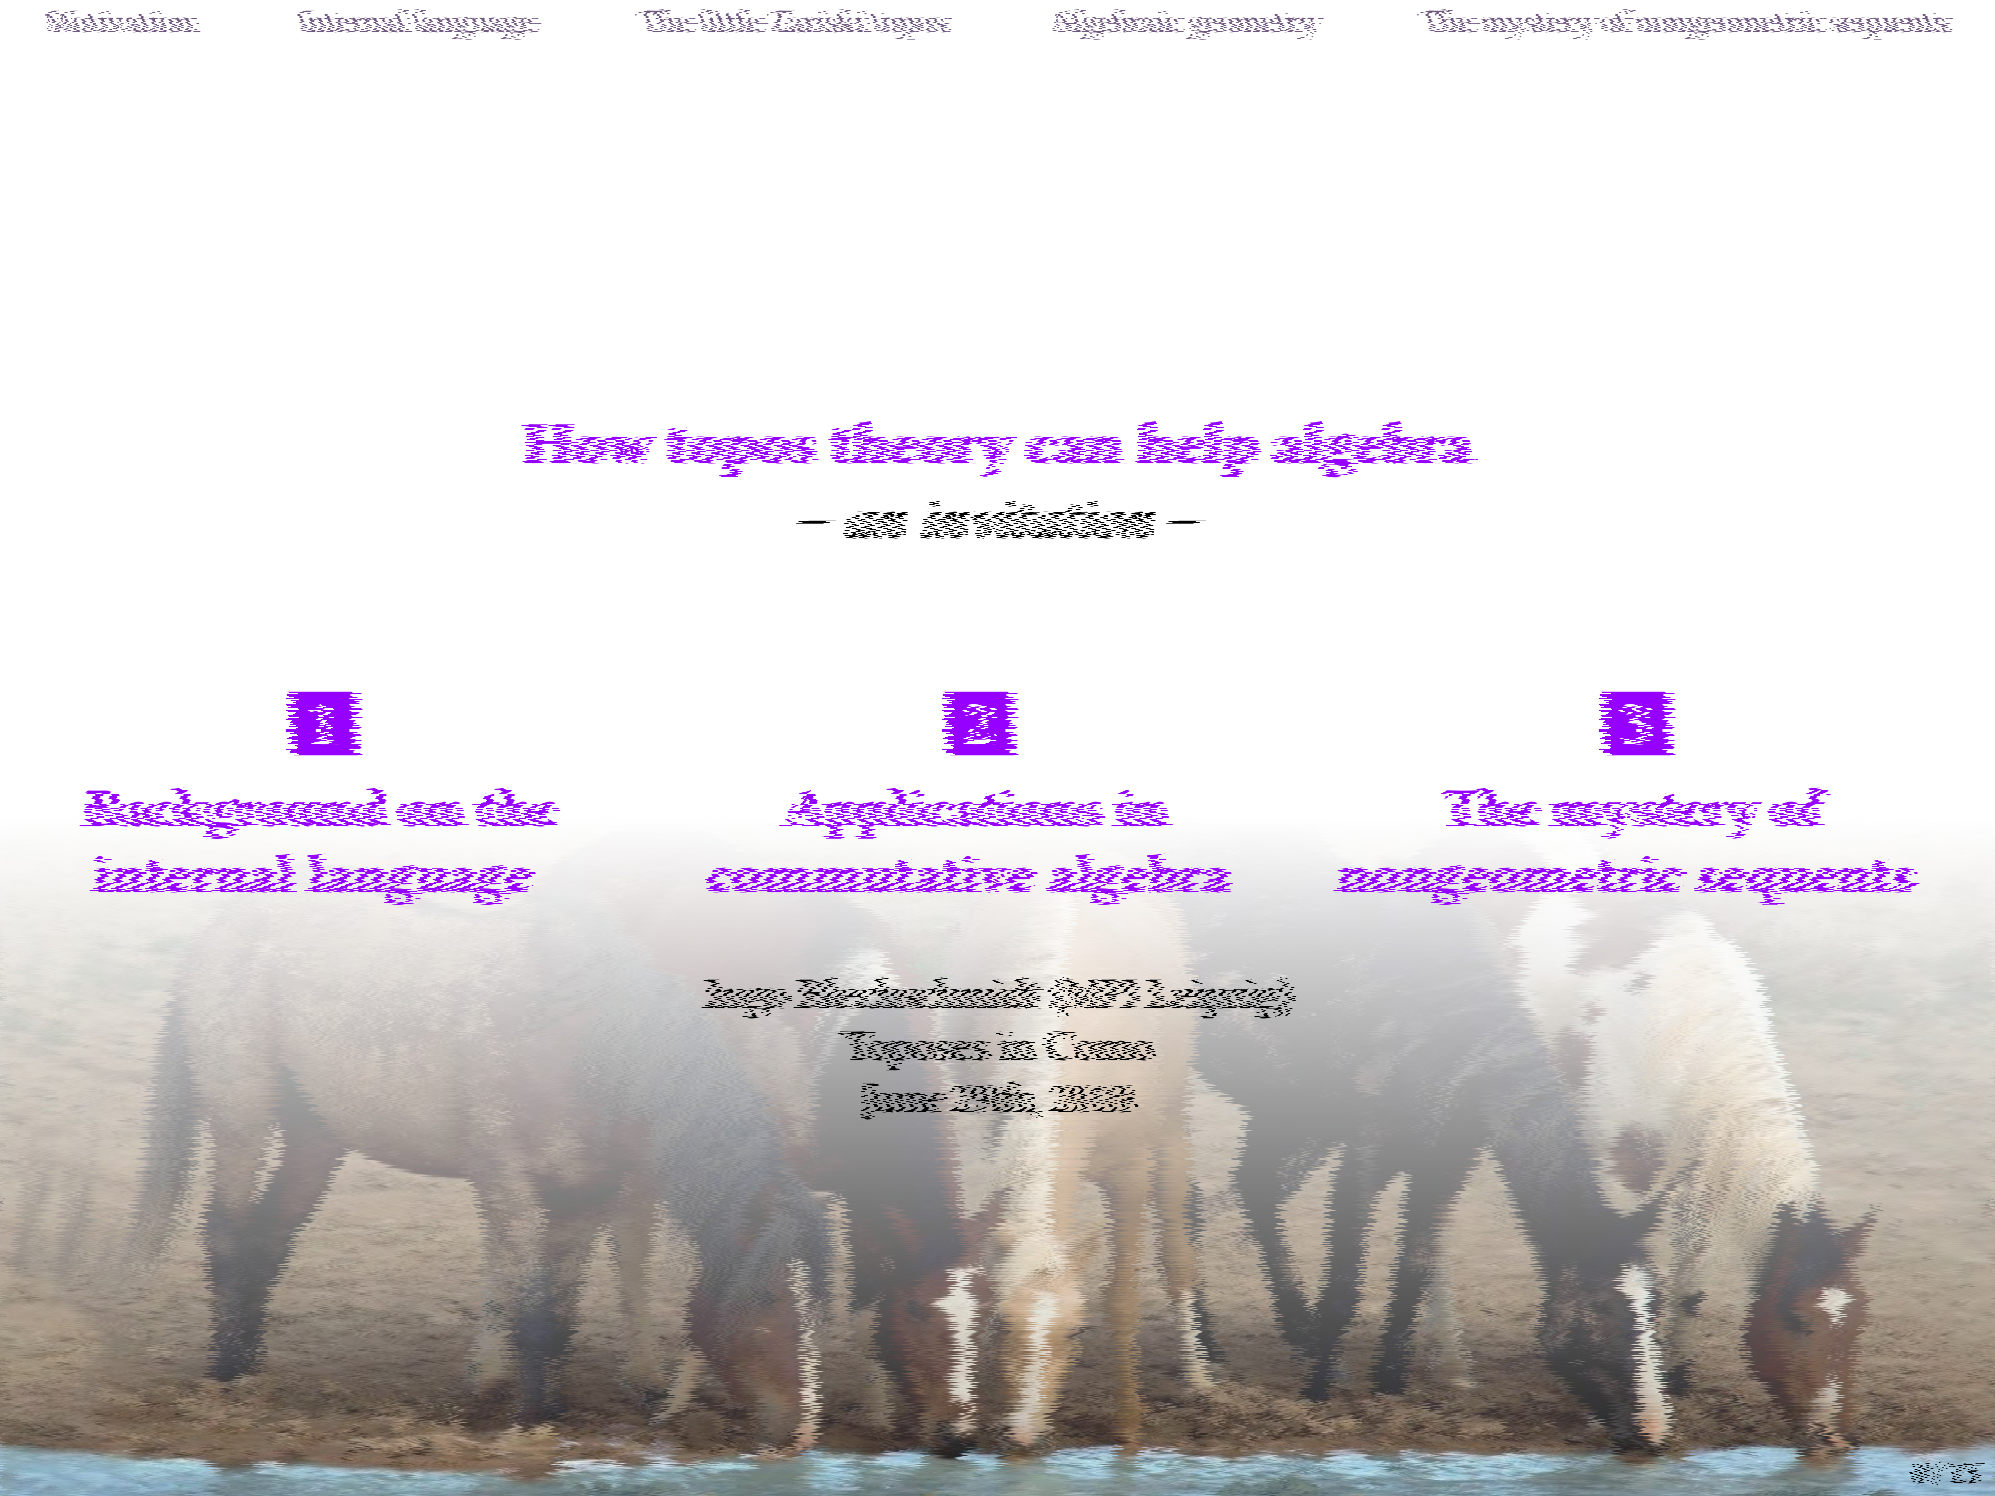
\includegraphics[width=\paperwidth]{slides-como2018-titlepage-blurred}}
%\begin{frame}[plain]\end{frame}}

\addtocounter{framenumber}{-1}

{\usebackgroundtemplate{\begin{minipage}{\paperwidth}\vspace*{4.95cm}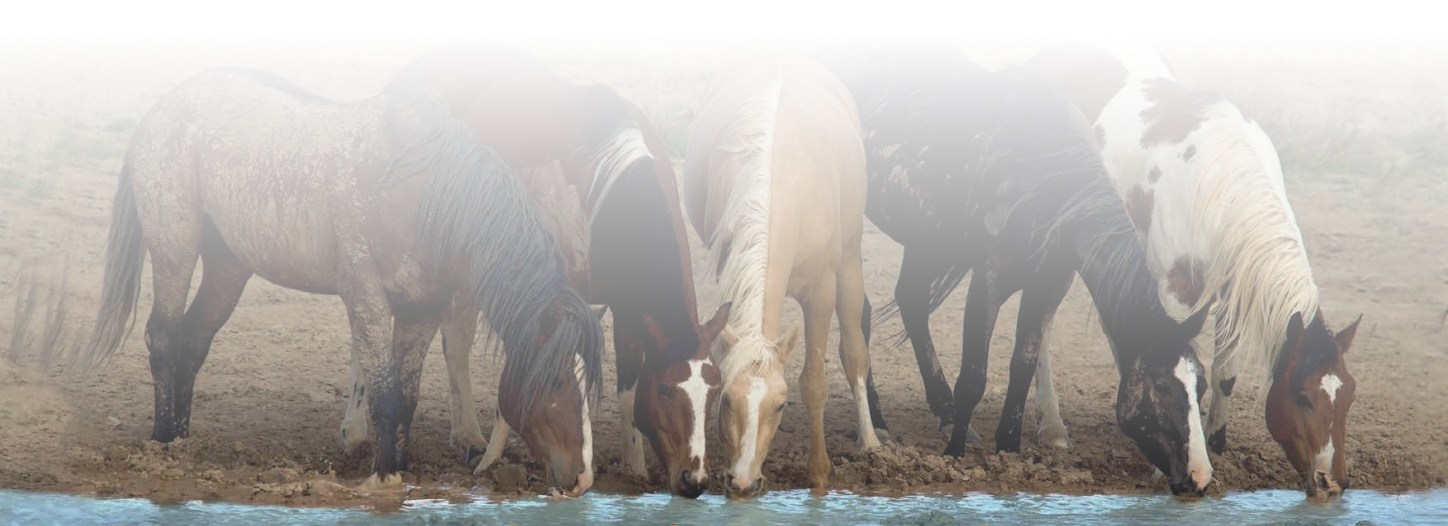
\includegraphics[width=\paperwidth]{topos-horses}\end{minipage}}
\begin{frame}[c]
  \centering
  \medskip
  \hspace*{-3.9em}%

  \hil{How topos theory can help commutative algebra} \\

  \emph{-- an invitation --}

  \bigskip
  \bigskip

  \begin{columns}
    \small
    \begin{column}{0.33\textwidth}
      \centering
      \bignumber{1}
      \smallskip

      \hil{Background on the internal language}
      \medskip
    \end{column}

    \begin{column}{0.33\textwidth}
      \centering
      \bignumber{2}
      \smallskip

      \hil{Applications in commutative algebra}
      \medskip
    \end{column}

    \begin{column}{0.33\textwidth}
      \centering
      \bignumber{3}
      \smallskip

      \hil{The mystery of \mbox{\!\!nongeometric sequents}}
      \medskip
    \end{column}
  \end{columns}

  \scriptsize
  Ingo Blechschmidt (MPI Leipzig) \\
  Toposes in Como \\
  June 29th, 2018
  \par
\end{frame}}


\section{Motivation}

\begin{frame}{Motivating testcases}
  Let $A$ be a ring (commutative, with unit, $1 = 0$ allowed). \\
  Assume that $A$ is reduced: If $x^n = 0$, then $x = 0$.

  \jnote{1-2}{The two displayed statements are trivial for fields. It is
  therefore natural to try to reduce the general situation to the field
  situation.}

  \jnote{2}{The displayed proofs, which could have been taken from any
  standard textbook on commutative algebra, succeed in this reduction quite
  easily by employing maximal ideals or minimal prime ideals. However, this way
  of reducing comes at a cost: It requires the Boolean Prime Ideal Theorem
  (for ensuring the existence of a prime ideal and for ensuring that stalks at
  minimal prime ideals are fields) and even the full axiom of choice (for
  ensuring the existence of a minimal prime ideal).

  It therefore doesn't work in the internal universe of most toposes, and in
  any case it obscures explicit computational content: Statements so simple as
  the two displayed ones should admit explicit, computational proofs.

  We'll learn how the internal language of a certain well-chosen topos provides
  a way to perform the reduction in an entirely constructive manner. If so
  desired, the resulting topos-theoretic proofs can be unwinded to yield fully
  explicit, topos-free, direct proofs.

  Beautiful constructive proofs can also be found in Richman's note on
  \fixedhref{https://www.ams.org/journals/proc/1988-103-04/S0002-9939-1988-0954974-5/S0002-9939-1988-0954974-5.pdf}{nontrivial
  uses of nontrivial rings} and in the
  \fixedhref{https://arxiv.org/abs/1605.04832}{recent textbook by Lombardi and
  Quitté} on constructive commutative algebra.}

  \jnote{3}{We can slightly reduce the requirements of the proof of the first
  statement by employing not a maximal ideal, but a prime ideal. The existence
  of maximal ideals is nontrivial rings is equivalent to the axiom of choice,
  while the existence of prime ideals is equivalent to the weaker Boolean Prime
  Ideal Theorem. However, this improvement doesn't change the main point; the
  proof is still wildly unconstructive.}

  \jnote{4-}{Grothendieck's generic freeness lemma is an important theorem in
  algebraic geometry, where it is usually stated in the following geometric
  form:
  \begin{indentblock}Let~$X$ be a reduced scheme. Let~$\B$ be
  an~$\O_X$-algebra of finite type. Let~$\M$ be a~$\B$-module of finite type.
  Then over a dense open,
  \begin{enumerate}
  \item[(a)] $\B$ and~$\M$ are locally free as sheaves of~$\O_X$-modules,
  \item[(b)] $\B$ is of finite presentation as a sheaf of~$\O_X$-algebras and
  \item[(c)] $\M$ is of finite presentation as a sheaf of~$\B$-modules.
  \end{enumerate}\end{indentblock}}

  \jnote{5}{All previously known proofs proceed in a series of reduction steps,
  finally culminating in the case where~$A$ is a Noetherian integral domain.
  They are somewhat convoluted (for instance, the proof in the Stacks Project
  is three pages long) and employ several results in commutative algebra which
  have not yet been constructivized.

  Using the internal language of toposes, we will give a short, conceptual and
  constructive proof of Grothendieck's generic freeness lemma. Again, if so
  desired, one can unwind the internal proof to obtain a
  constructive proof which doesn't reference topos theory. The proof obtained
  in this way is still an improvement on the previously known proofs, requiring
  no advanced prerequisites in commutative algebra, and takes
  \fixedhref{https://arxiv.org/abs/1807.01231}{about
  a page}.}

  \only<1-3>{\begin{columns}[t]
  \begin{column}[t]{0.50\textwidth}
    \centering

    \scalebox{0.8}{$\begin{pmatrix}
      \cdot & \cdot \\
      \cdot & \cdot \\
      \cdot & \cdot
      \end{pmatrix}$}
    \vspace*{-1em}

    \begin{varblock}{\textwidth}{A baby application}
      \justifying
      Let~$M$ be a surjective matrix over~$A$ with more rows than columns.
      Then~$1 = 0$ in~$A$.
    \end{varblock}

    \justifying
    \only<2>{\textbf{Proof.} \bad{Assume not.} Then there is~a \bad{maximal
    ideal} $\mmm$. The matrix is surjective over the field~$A/\mmm$. This is a
    contradiction to basic linear algebra.}

    \only<3>{\textbf{Proof.} \bad{Assume not.} Then there is~a \bad{prime
    ideal} $\ppp$. The matrix is surjective over the
    field~$\mathrm{Quot}(A/\ppp)$. This is a contradiction to basic linear
    algebra.}
  \end{column}

  \begin{column}[t]{0.5\textwidth}
    \centering

    \scalebox{0.8}{$\begin{pmatrix}
      \cdot & \cdot & \cdot & \cdot \\
      \cdot & \cdot & \cdot & \cdot \\
      \cdot & \cdot & \cdot & \cdot
    \end{pmatrix}$}
    \vspace*{-1em}

    \begin{varblock}{\textwidth}{A child application}
      \justifying
      Let~$M$ be an injective matrix over~$A$ with more columns than rows.
      Then~$1 = 0$ in~$A$.
    \end{varblock}

    \justifying
    \visible<2-3>{\textbf{Proof.} \bad{Assume not.} Then there is a \bad{minimal
    prime ideal} $\ppp$. The matrix is injective over the field~$A_\ppp = A[(A
    \setminus \ppp)^{-1}]$. This is a contradiction to basic linear algebra.}
    \end{column}
  \end{columns}}

  \pause
  \pause
  \pause

  \centering

  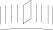
\includegraphics[height=3em]{generic-freeness}
  \vspace*{-1em}

  \begin{varblock}{0.9\textwidth}{Generic freeness$\phantom{p}$}
    \justifying
    Let~$B$ be an~$A$-algebra of finite type ($\cong A[X_1,\ldots,X_n]/\aaa$). \\
    Let~$M$ be a finitely generated~$B$-module ($\cong B^m/U$).

    If~$f = 0$ is the only element of~$A$ such that
    \begin{enumerate}
      \item $B[f^{-1}]$ and $M[f^{-1}]$ are free modules over $A[f^{-1}]$,
      \item $A[f^{-1}] \to B[f^{-1}]$ is of finite presentation and
      \item $M[f^{-1}]$ is finitely presented as a module over~$B[f^{-1}]$,
    \end{enumerate}
    then $1 = 0$ in~$A$.
  \end{varblock}
  \vspace*{-0.5em}

  \pause\center
  \begin{minipage}{0.9\textwidth}
    \textbf{Proof.} See [Stacks Project, Tag 051Q].
  \end{minipage}
\end{frame}


\section{Internal language}

\begin{frame}{The internal language of a topos}
  For any topos~$\E$ and any formula~$\varphi$, we define the meaning of
  \vspace*{-0.5em}
  \[
    \text{``$\E \models \varphi$''} \quad
    \text{(``$\varphi$ holds in the internal universe of~$\E$'')}
  \]

  \vspace*{-1.0em}
  using (Shulman's extension of) the \hil{Kripke--Joyal semantics}.

  \jnote{1}{The internal language of a topos allows to construct objects and
  morphisms, formulate statements about them and prove such statements in a
  naive element-based language. From the internal point of view, objects look
  like sets [more precisely, types]; morphisms look like maps; epimorphisms
  look like surjections; group objects look like groups; and so on.

  To determine whether a statement~$\varphi$ holds in the internal universe of a
  given topos, one can use the Kripke--Joyal semantics to translate it into an
  ordinary external statement and then check the validity of the external
  translation.

  For instance, in the ef{}fective topos the curious statement~``any function
  $\NN \to \NN$ is computable'' holds, for its external meaning is the
  triviality ``there is a Turing machine which given a Turing machine computing
  some function~$f : \NN \to \NN$ outputs a Turing machine computing~$f$''. In
  contrast, the statement~``any function~$\NN \to \NN$ is either the zero
  function or not'' does not hold in the ef{}fective topos, since its external
  meaning is ``there exists a Turing machine which given a Turing machine
  computing some function~$f : \NN \to \NN$ decides whether~$f$ is the zero
  function or not''.}

  \jnote{2}{Any theorem which has an intuitionistic proof holds in
  the internal universe of any topos. The restriction to intuitionistic logic
  is not due to philosophical concerns; it is a fact of life that only very few
  toposes validate the law of excluded middle (for instance, sheaf toposes over
  discrete topological space do if the law of excluded middle is available in
  the metatheory). Luckily, vast amounts of mathematics can be developed in a
  purely intuitionistic setting.

  The internal language machinery itself can be developed in an intuitionistic
  setting.

  The standard internal language of toposes in not enough for our purposes, as
  it misses unbounded quantification (``for all groups'', ``for all rings'')
  and dependent types. Shulman's \fixedhref{https://arxiv.org/abs/1004.3802}{stack
  semantics} offers what we need. No knowledge of stacks is necessary to enjoy
  his paper. Prior work includes
  \fixedhref{https://www.cl.cam.ac.uk/~amp12/papers/polist/polist.pdf}{Polymorphism
  is Set Theoretic, Constructively} by Pitts and
  \fixedhref{http://www.phil.cmu.edu/projects/ast/Papers/Awodey-Butz-Simpson-Streicher-APAL-2013.pdf}{Relating
  first-order set theories, toposes and categories of classes} by Awodey, Butz,
  Simpson and Streicher (obtained independently and published after Shulman).}

  \vspace*{-1em}
  \begin{columns}
    \def\insertblocktitle{}
    \begin{column}{0.25\textwidth}\usebeamertemplate{block begin}
      \centering
      $\Set \models \varphi$ \\
      ``$\varphi$ holds in the \\ usual sense.''
      \usebeamertemplate{block end}\end{column}

    \begin{column}{0.25\textwidth}\usebeamertemplate{block begin}
      \centering
      $\Sh(X) \models \varphi$ \\
      ``$\varphi$ holds continuously.''
      \usebeamertemplate{block end}\end{column}

    \begin{column}{0.25\textwidth}\usebeamertemplate{block begin}
      \centering
      $\Eff \models \varphi$ \\
      ``$\varphi$ holds \\ computably.''
      \usebeamertemplate{block end}\end{column}
  \end{columns}
  \medskip

  Any topos supports \hil{mathematical reasoning}:

  \vspace*{-1.5em}
  \begin{hilblock}
    If~$\E \models \varphi$ and if~$\varphi$ entails~$\psi$
    \pointthis{<2>}{intuitionistically}{%
      no $\varphi \vee \neg\varphi$,\ \
      no $\neg\neg\varphi \Rightarrow \varphi$,\ \
      no axiom of choice},
    then~$\E \models \psi$.
  \end{hilblock}
\end{frame}

\begin{frame}{The Kripke--Joyal semantics of~$\boldsymbol{\Sh(X)}$}
  \small\vspace*{-0.5em}
  Let~$X$ be a topological space. We recursively define
  \[ U \models \varphi \quad \text{(``$\varphi$ holds on~$U$'')} \]
  \mbox{for open subsets~$U \subseteq X$ and formulas~$\varphi$.
  Write~``$\Sh(X) \models \varphi$'' to mean~$X \models \varphi$.}
  \footnotesize
  \[ \renewcommand{\arraystretch}{1.08}\begin{array}{@{}l@{\ }c@{\ }l@{}}
  U \models \top &\Ll& \text{true} \\
  U \models \bot &\Ll& \hcancel{\text{false}}{0pt}{3pt}{0pt}{-2pt}\ U = \emptyset \\
  U \models s = t \? F &\Ll& s|_U = t|_U \in F(U) \\
  U \models \varphi \wedge \psi &\Ll&
  \text{$U \models \varphi$ and $U \models \psi$} \\
  U \models \varphi \vee \psi &\Ll&
  \hcancel{\text{$U \models \varphi$ or $U \models \psi$}}{0pt}{3pt}{0pt}{-2pt}\ \text{there exists a covering $U = \bigcup_i U_i$} \\
  && \quad\quad\text{such that for all~$i$: $U_i \models \varphi$ or $U_i \models \psi$} \\
  U \models \varphi \Rightarrow \psi &\Ll&
  \text{for all open~$V \subseteq U$: }
  \text{$V \models \varphi$ implies $V \models \psi$} \\
  U \models \forall s \? F\_ \varphi(s) &\Ll&
  \text{for all open $V \subseteq U$ and sections~$s_0 \in F(V)$: $V \models \varphi(s_0)$} \\
  U \models \forall F\_ \varphi(F) &\Ll&
  \text{for all open $V \subseteq U$ and sheaves~$F_0$ over~$V$: $V \models \varphi(F_0)$} \\
  U \models \exists s \? F\_ \varphi(s) &\Ll&
  \hcancel{\text{there exists $s_0 \in F(U)$ such that $U \models \varphi(s_0)$}}{0pt}{3pt}{0pt}{-2pt} \\
  && \quad\quad
  \text{there exists a covering $U = \bigcup_i U_i$ such that for all~$i$:} \\
  && \quad\quad\quad\quad \text{there exists~$s_0 \in F(U_i)$ such that $U_i \models \varphi(s_0)$} \\
  U \models \exists F\_ \varphi(F) &\Ll&
  \hcancel{\text{there exists a sheaf $F_0$ on $U$ such that $U \models
  \varphi(F_0)$}}{0pt}{3pt}{0pt}{-2pt} \\
  && \quad\quad
  \text{there exists a covering $U = \bigcup_i U_i$ such that for all~$i$:} \\
  && \quad\quad\quad\quad \text{there exists a sheaf~$F_0$ on $U_i$ such that $U_i \models \varphi(F_0)$}
  \end{array} \]

  \jnote{1}{Many interesting sheaves have few global sections, which is why a
  definition should as ``$U \models \forall s \? F\_ \varphi(s)$ iff $U \models
  \varphi(s_0)$ for all~$s_0 \in F(U)$'' would miss the point. More precisely,
  changing the definitions like this would yield the internal language of the
  topos of presheaves on~$X$.

  Here is an explicit example of the translation procedure. Let~$\alpha : F
  \to G$ be a morphism of sheaves on~$X$. Then (the corner quotes ``$\speak{\ldots}$''
  indicate that translation into formal language is left to the reader):
  \footnotesize
  \begin{align*}
    & X \models \speak{$\alpha$ is injective} \\[0.2em]
    \Longleftrightarrow\
    & X \models \forall s\?F\_ \forall t\?F\_ \alpha(s) = \alpha(t) \Rightarrow s = t \\[0.2em]
    \Longleftrightarrow\ &
      \text{for all open~$U \subseteq X$, sections $s_0 \in F(U)$:} \\
    &\qquad\qquad
        U \models \forall t\?F\_ \alpha(s_0) = \alpha(t) \Rightarrow s_0 = t \\[0.2em]
    \Longleftrightarrow\ &
      \text{for all open~$U \subseteq X$, sections $s_0 \in F(U)$:} \\
    &\qquad\qquad
        \text{for all open~$V \subseteq U$, sections $t_0 \in F(V)$:} \\
    &\qquad\qquad\qquad\qquad
          V \models \alpha(s_0) = \alpha(t_0) \Rightarrow s_0 = t_0 \\[0.2em]
    \Longleftrightarrow\ &
      \text{for all open~$U \subseteq X$, sections $s_0 \in F(U)$:} \\
    &\qquad\qquad
        \text{for all open~$V \subseteq U$, sections $t_0 \in F(V)$:} \\
    &\qquad\qquad\qquad\qquad
          \text{for all open $W \subseteq V$: $\alpha_V(s_0|_W) = \alpha_V(t_0|_W)$ implies $s_0|_W = t_0|_W$} \\[0.2em]
    \Longleftrightarrow\ &
      \text{for all open~$U \subseteq X$, sections $s, t \in F(U)$:
        $\alpha_U(s|_U) = \alpha_U(t|_U)$ implies $s|_U = t|_U$} \\[0.2em]
    \Longleftrightarrow\ &
      \text{$\alpha$ is a monomorphism of sheaves}
  \end{align*}}
\end{frame}

\begin{frame}{Internalizing parameter-dependence}
  \justifying
  Let~$X$ be a space. A continuous family~$(f_x)_{x \in X}$ of continuous
  functions (that is, a continuous function~$f : X \times \RR \to \RR$;
  $f_x(a) = f(x,a)$) induces an endomorphism of the sheaf~$\C$ of continuous
  functions:
  \[
    \bar f : \C \longrightarrow \C,\
    \text{on $U$:}\ s \longmapsto (x \mapsto f_x(s(x))).
  \]

  \vspace*{-1em}

  \begin{itemize}
    \item $\Sh(X) \models \speak{The set $\C$ is the set of (Dedekind) reals}$.
    \item $\Sh(X) \models \speak{The function $\bar f : \RR \to \RR$ is continuous}$. \bigskip
    \item Iff $f_x(-1) < 0$ for all $x$, then $\Sh(X) \models \bar f(-1) < 0$.
    \item Iff $f_x(+1) > 0$ for all $x$, then $\Sh(X) \models \bar f(+1) > 0$.
    \item Iff all $f_x$ are increasing, then $\Sh(X) \models \speak{$\bar f$ is
    increasing}$. \bigskip
    \item \ \\[-1.2em]\mbox{Iff there is an open cover~$X = \bigcup_i U_i$ such
    that for each~$i$ there is a} \mbox{continuous function~$s : U_i \to \RR$
    with~$f_x(s(x)) = 0$ for all~$x \in U_i$,} then $\Sh(X) \models \exists s
    \? \RR\_ \bar f(s) = 0$.
  \end{itemize}

  \jnote{1}{This slide, unrelated to commutative algebra or algebraic geometry,
  aims to illustrate one of the basic uses of the internal language of toposes:
  Upgrading any theorem admitting an intuitionistic proof to a
  parameter-dependent version.

  Constructively, there are several non-equivalent forms of the intermediate
  value theorem. The following version doesn't admit an intuitionistic proof:
  \begin{indentblock}Let~$g : \RR \to \RR$ be a function between the (Dedekind)
  reals which is continuous in the usual epsilon/delta sense. Assume~$g(-1) < 0
  < g(1)$. Then there exists a number~$x \in \RR$ such that~$g(x) = 0$.
  \end{indentblock}
  If there was an intuitionistic proof, the statement would hold in any topos,
  so in particular in sheaf toposes over topological spaces. By the
  translations shown on the slide, this
  would amount to the following strengthening of the intermediate value
  theorem: In continuous families of continuous functions, zeros can locally be
  picked continuously. However, this strengthening is invalid, as
  \fixedhref{https://raw.githubusercontent.com/iblech/internal-methods/master/images/zeros-in-families.mp4}{this
  video shows}.

  \centering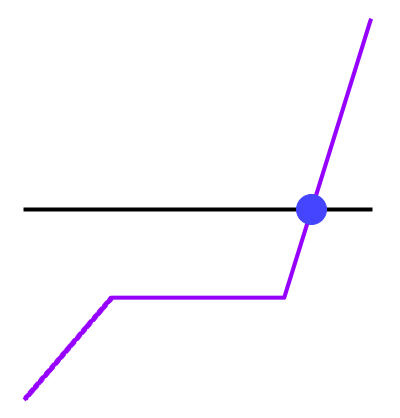
\includegraphics[width=0.1\textwidth]{zeros-in-families-still}}

  \jnote{2}{In contrast, the following version does admit an intuitionistic
  proof. We can therefore interpret it in sheaf toposes over topological
  spaces and thereby obtain the strengthening that in continuous families of
  strictly increasing continuous functions, zeros can locally be picked
  continuously. You are invited to prove this strengthening directly, without
  reference to the internal language.
  \begin{indentblock}Let~$g : \RR \to \RR$ be a function between the (Dedekind)
  reals which is continuous in the usual epsilon/delta sense and which is
  strictly increasing ($a < b$ implies~$g(a) < g(b)$). Assume~$g(-1) < 0 <
  g(1)$. Then there exists a number~$x \in \RR$ such that~$g(x) =
  0$.\end{indentblock}}
\end{frame}


\section{The little Zariski topos}

\begin{frame}{The little Zariski topos}
  Let~$A$ be a ring. Its \hil{little Zariski topos} is equivalently
  \begin{enumerate}
    \item the classifying topos of \hil{local localizations} of $A$,
    \item the classifying locale of \hil{prime filters} of $A$,
    \item the locale given by the frame of \hil{radical ideals} of $A$,
    \item the topos of sheaves over the poset $A$ with $f \preceq g$ iff $f \in \sqrt{(g)}$ and with $(f_i \to f)_i$ deemed covering iff $f \in \sqrt{(f_i)_i}$ or
    \item the topos of sheaves over $\Spec(A)$.
  \end{enumerate}
  Its associated topological space of points is the \hil{classical spectrum}
  \[ \{ \fff \subseteq A \,|\, \text{$\fff$ prime filter} \} + \text{Zariski topology}. \]
  It has \hil{enough points} if the Boolean Prime Ideal Theorem holds.

  \footnotesize
  Prime ideal:\, $0 \in \ppp$;\, $x \in \ppp \wedge y \in \ppp \Rightarrow x+y \in \ppp$;\, $1 \not\in \ppp$;\, $xy \in \ppp \Leftrightarrow x \in \ppp \vee y \in \ppp$

  Prime filter:\, $0 \not\in \fff$;\,\,
  $x+y \in \fff \Rightarrow x \in \fff \vee y \in \fff$;
  \hspace*{0.5pt}\,\,
  $1 \in \fff$;\,
  $xy \in \fff \Leftrightarrow x \in \fff \wedge y \in \fff$

  \jnote{1}{Any geometric theory has a classifying topos; if the theory under
  consideration is propositional (doesn't have any sorts), then its classifying
  topos can be chosen to be the topos of sheaves over a locale. One can also
  give a direct account of classifying locales, as a pedagogical stepping stone
  to the full theory of classifying toposes.

  The slide contains a small lie: The classical definition of the spectrum of a
  ring is via the set of prime ideals of~$A$, not prime filters. If the law of
  excluded middle is available, there is no difference between these
  definitions since the complement of a prime ideal is a prime filter and vice
  versa.

  One can also consider the classifying local of prime \emph{ideals} of~$A$.
  Its associated topological space of points is the the set of prime ideal
  of~$A$ equipped with the \emph{constructible topology}.

  In an intuitionistic context, any of the (generalized) spaces of items~1--4
  can be adopted as sensible definitions of the spectrum of~$A$. Item~5 is then
  a tautology. The classical definition of the spectrum as a topological space
  doesn't work very well, because verifying the universal property one expects
  of it requires the Boolean Prime Ideal Theorem. Most dramatically, there are
  rings which are not trivial yet have neither prime ideals nor prime filters.
  The classical definition yields in this case the empty space.}
\end{frame}

\begin{frame}{First steps in the little Zariski topos}
  Let~$A$ be a ring. Let~$\fff_0$ be the \hil{generic prime filter} of~$A$; it
  is a subobject of the constant sheaf~$\ull{A}$ of the little Zariski topos.

  \begin{itemize}
    \item The ring $A^\sim \defeq \ull{A}[\fff_0^{-1}]$ is the generic local
    localization of $A$.
    \item Given an~$A$-module~$M$, we have the~$A^\sim$-module $M^\sim \defeq
    \ull{M}[\fff_0^{-1}]$.
  \end{itemize}

  \jnote{1}{The Kripke--Joyal semantics for the little Zariski topos amounts to
  the following: $\Spec(A) \models \varphi$ iff~$D(1) \models \varphi$, and the
  clauses for~$D(f) \models \varphi$, where~$f$ ranges over the elements
  of~$A$, are given by the following table.
  \[\footnotesize\renewcommand{\arraystretch}{1.25}\begin{array}{@{}l@{\quad}c@{\quad}l@{}}
    D(f) \models \top &\text{iff}& \text{true} \\
    D(f) \models \bot &\text{iff}& \text{$f$ is nilpotent} \\
    D(f) \models x = y &\text{iff}& x = y \in A[f^{-1}] \\
    D(f) \models \varphi \wedge \psi &\text{iff}&
      \text{$D(f) \models \varphi$ and $D(f) \models \psi$} \\
    D(f) \models \varphi \vee \psi &\text{iff}&
      \text{there exists a partition~$f^n = fg_1 + \cdots + fg_m$ with,} \\
    &&\quad\text{for each~$i$, $D(fg_i) \models \varphi$ or $D(fg_i) \models \psi$} \\
    D(f) \models \varphi \Rightarrow \psi &\text{iff}&
      \text{for all~$g \in A$, $D(fg) \models \varphi$ implies $D(fg) \models \psi$} \\
    D(f) \models \forall x\?M^\sim\_ \varphi(x) &\text{iff}&
      \text{for all~$g \in A$ and $x_0 \in M[(fg)^{-1}]$, $D(fg) \models \varphi[x_0/x]$} \\
    D(f) \models \exists x\?M^\sim\_ \varphi(x) &\text{iff}&
      \text{there exists a partition~$f^n = fg_1 + \cdots + fg_m$ with,} \\
    &&\quad\text{for each~$i$, $D(fg_i) \models \varphi[x_0/x]$ for some~$x_0 \in M[(fg_i)^{-1}]$}
  \end{array} \]
  The generic prime filter~$\fff_0$ can also be described in explicit
  terms. For ring elements~$f$ and~$s$, $D(f) \models (s \in \fff_0)$ iff~$f
  \in \sqrt{(s)}$.}

  \jnote{2}{Our description of~$M^\sim$ reveals a precise sense in
  which~$M^\sim$ and~$M$ are related: $M^\sim$ is simply a localization of~$M$
  (first lifted to another universe by the constant sheaf construction). The
  classical descriptions don't make the relation evident.

  As a first approximation, the module~$M^\sim$ can be thought of as a
  reification of all the stalks of~$M$ as a single object. The metatheorem
  displayed at the top left on the next slides makes this precise and also
  exposes the limits of this view: It is only correct for geometric sequents.
  When considering nongeometric sequents, phenomena appear which are unique
  to~$M^\sim$ in the sense that they are in general not shared by~$M$, its
  stalks or its quotients.}

  \jnote{3}{One can show, assuming that the little Zariski topos is
  \emph{overt}, that the module~$M$ in~$\Set$ and the module~$\ull{M}$ of the
  little Zariski topos share all first-order properties. This observation
  explains the metatheorem displayed at the bottom left. The assumption is
  satisfied if any element of~$A$ is nilpotent or not nilpotent, so it's always
  satisfied if the law of excluded middle is available in the metatheory. In an
  intuitionistic context, it's still ``morally satisfied''. Details are in
  Section~12.9 of
  \fixedhref{https://rawgit.com/iblech/internal-methods/master/notes.pdf}{these
  notes}.

  The metatheorem soups up a number of lemmas of algebraic geometry, there
  stated in geometric language. For instance, if~$M$ is finitely generated,
  then~$M^\sim$ is of finite type. If~$M$ is finitely presented, then~$M^\sim$
  is of finite presentation. If~$M$ is coherent, then~$M^\sim$ is coherent.

  As an aside, the little Zariski topos is seldomly Boolean (validates the law of
  excluded middle). A necessary condition is that~$A$ is of dimension~$\leq 0$.}

  \jnote{4}{Assuming that~$A$ is reduced, the following nongeometric sequents
  hold in the little Zariski topos (among others):

  $A^\sim$ is a field in the sense that zero is the only noninvertible
  element. This field property was already observed in the 1970s by Mulvey, who
  didn't know a deeper reason for this property. We now know that it's a
  shadow of an internal property whose external translation expresses
  that~$A^\sim$ is quasicoherent.

  $A^\sim$ has~$\neg\neg$-stable equality in the sense that
  \[ \Spec(A) \models \forall s\?A^\sim\_ \neg\neg(s = 0) \Rightarrow s = 0. \]
  Classically, every set has~$\neg\neg$-stable equality; intuitionistically,
  this is a special property of some sets. It's quite useful, as some theorems
  of classical commutative algebra can only be proven intuitionistically when
  weakened by double negation. The stability then allows, in some cases, to
  obtain the original conclusion.

  $A^\sim$ is anonymously Noetherian in the sense that any of its ideals
  is \mbox{\emph{not not}} finitely generated. A philosophically-motivated
  constructivist might be offended by this notion, since it runs counter to the
  maxim that constructive mathematics should be informative. However, in the
  internal context it is a useful notion: Hilbert's basis theorem holds for it,
  and we'll put it to good use in our proof of Grothendieck's generic freeness
  lemma.}

  \jnote{5}{Are there theorems which can only be proven using the internal
  language and not be proven without?

  No. Just as the translation from internal statements to external statements
  is entirely mechanical, so is the translation from internal proofs to
  external proofs. Any proof employing the internal language can be unwinded to
  yield an external proof not referencing the internal language.

  However, depending on the logical complexity of the statements occuring in a
  given proof, the resulting external proof might be (much) more complex than
  the internal proof. This is particularly the case if the proof involves
  double negation, for much the same reason as that in computer science,
  continuations can twist the control flow in nontrivial ways which are
  sometimes hard to understand. It is in these cases where we can extract the
  most value of the internal language, unlocking notions and proofs which might
  otherwise be hard to obtain.

  The slide shows a specific example. The internal statement
  that~$A^\sim[X_1,\ldots,X_n]$ is anonymously Noetherian is quite simple; its
  external translation is quite convoluted.}

  \pause
  \only<2>{\begin{center}
    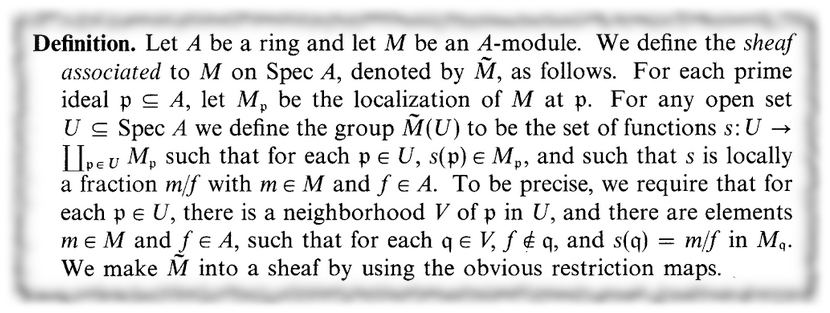
\includegraphics[width=0.9\textwidth]{hartshorne-tilde-construction} \\
    \footnotesize
    Robin Hartshorne. Algebraic Geometry. 1977.
  \end{center}}
  \pause

  \vspace*{-1.5em}

  \begin{columns}
    \begin{column}{0.48\textwidth}
      \begin{varblock}{\textwidth}{}
        \justifying
        Assuming the Boolean prime ideal theorem, a geometric sequent
        ``$\forall \ldots \forall\_ (\cdots \Longrightarrow \cdots\!\,)$'',
        where the two subformulas may not contain~``$\Rightarrow$'' and~``$\forall$'',
        holds for~$M^\sim$ iff it holds for all stalks~$M_\ppp$.
      \end{varblock}

      \vspace*{-1.5em}

      \begin{varblock}{\textwidth}{}
        $M^\sim$ inherits any property of~$M$ which is \hil{localization-stable}.
      \end{varblock}
    \end{column}

    \begin{column}{0.5\textwidth}
      \vspace*{1.5em}

      If $A$ is reduced ($x^n = 0 \Rightarrow x = 0$):

      \vspace*{-1.0em}

      \setbeamercolor{block body}{bg=red!30}
      \setbeamercolor{structure}{fg=purple}
      \begin{varblock}{\textwidth}{}
        $A^\sim$ is a \hil{field}
        (nonunits are zero).

        $A^\sim$ has \hil{$\boldsymbol{\neg\neg}$-stable equality}.

        \mbox{$A^\sim$ is \hil{anonymously Noetherian}.}\\[-1.2em]
      \end{varblock}
    \end{column}
  \end{columns}

  \visible<4-5>{\begin{tikzpicture}[overlay]
    \draw[fill=white, draw=white, opacity=0.95] (-1,0) rectangle (\paperwidth,7.4);
    \node[anchor=south west,inner sep=0] (image) at (0,0.8) {\vbox{
      \only<4>{
	\centering
	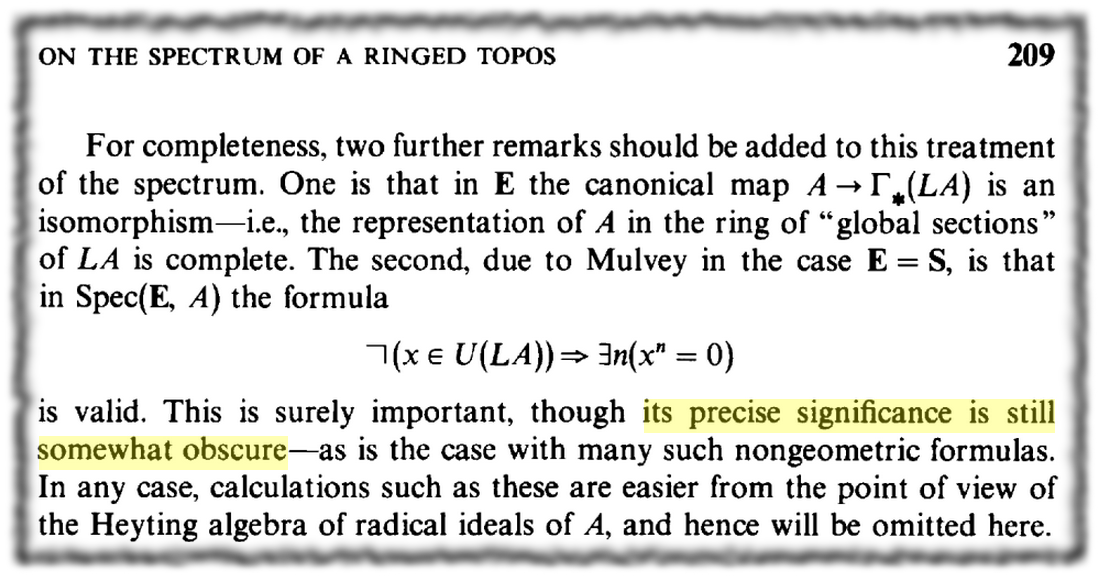
\includegraphics[width=0.9\textwidth]{tierney-on-the-spectrum-of-a-ringed-topos} \\
	\footnotesize
	Miles Tierney. On the spectrum of a ringed topos. 1976.
      }

      \only<5>{
	\begin{varblock}{\textwidth}{Complexity reduction}
	  The external meaning of
	  \[
	    \Spec(A) \models
	      \speak{$A^\sim[X_1,\ldots,X_n]$ is anonymously Noetherian}
	  \]
	  is:
	  \medskip

	  \begin{indentblock}
	  For any element~$f \in A$ and any (not necessarily quasicoherent) sheaf of
	  ideals~$\J \hookrightarrow A^\sim[X_1,\ldots,X_n]|_{D(f)}$: If
	  \begin{indentblock}
	  for any element~$g \in A$ the condition that
	  \begin{indentblock}
	  the sheaf~$\J$ is of finite type on~$D(g)$
	  \end{indentblock}
	  implies that~$g = 0$,
	  \end{indentblock}
	  then~$f = 0$.
	  \end{indentblock}
	\end{varblock}

	\vspace*{-2em}
      }
    }};
  \end{tikzpicture}}
\end{frame}

\begin{frame}{Revisiting the testcases}
  Let $A$ be a reduced ring.

  \jnote{1}{This slide delivers on the promise made earlier: Using the internal
  language of the little Zariski topos, we can reduce to the case of fields
  without having to employ maximal ideals, prime ideals or minimal prime ideals.
  Since the internal language machinery is itself constructive, the displayed
  proofs can be unwinded to yield external constructive proofs which don't
  reference topos theory. Details on these external proofs can soon be found in
  a forthcoming paper titled
  \fixedhref{https://rawgit.com/iblech/internal-methods/master/paper-wlog.pdf}{Without
  loss of generality, any reduced ring is a field}.}

  \jnote{2}{The testcase of Grothendieck's generic freeness lemma illustrates
  that the internal language of toposes can help commutative algebra even if
  one is not interested in constructivity issues. The previously known proofs
  are somewhat long and somewhat convoluted; the new proof is arguably short
  and simple.

  Details on the internal proof are in Section~11.5 of
  \fixedhref{https://rawgit.com/iblech/internal-methods/master/notes.pdf}{these
  notes}. The
  \fixedhref{https://arxiv.org/abs/1807.01231}{external
  proof} obtained by unwinding the internal one is still quite direct, compared
  to the previously published proofs, and interestingly follows a curious
  course: It starts with verifying, in an inductive manner, that~$B$ and~$M$
  are free; that~$A \to B$ is of finite presentation; and that~$M$ is finitely
  presented as a~$B$-module. Then the assumption for~$f = 1$ is used, rendering
  the prior steps moot, since over the zero ring any module is free and any
  algebra is of finite presentation. External translations of internal proofs
  which use double negation will always take such a course.}

  \jnote{3}{Here's a rough sketch why the double negations occur. In
  undergraduate linear algebra, we learn that any finitely generated vector
  space is free (has a basis), by the following argument:
  Let~$(v_1,\ldots,v_n)$ be a generating family. Either one of the generators can
  be expressed as a linear combination of the others or not. In the latter
  case, the family is linearly independent and we're done. In the former, we
  remove the redundant generator and continue by induction.

  This argument relies on the law of excluded middle and can therefore not put
  to work in the internal universe as is. However, intuitionistically we do
  have the weaker statement~$\neg\neg(\varphi \vee \neg\varphi)$, and we can
  use this law in place of the law of excluded middle to intuitionistially
  deduce that any finitely generated vector space does \emph{not not} have a
  basis.}

  \only<1>{\begin{columns}[t]
    \begin{column}[t]{0.47\textwidth}
      \centering

      \scalebox{0.8}{$\begin{pmatrix}
        \cdot & \cdot \\
        \cdot & \cdot \\
        \cdot & \cdot
        \end{pmatrix}$}
      \vspace*{-1em}

      \begin{varblock}{\textwidth}{A baby application}
        \justifying
        Let~$M$ be a surjective matrix over~$A$ with more rows than columns.
        Then~$1 = 0$ in~$A$.
      \end{varblock}

      \justifying
      \textbf{Proof.} The matrix is surjective over the field~$A^\sim$.
      This is a contradiction to basic linear algebra. Hence $\Spec(A) \models
      \bot$, thus $1 = 0$ in $A$.
    \end{column}
    \begin{column}[t]{0.47\textwidth}
      \centering

      \scalebox{0.8}{$\begin{pmatrix}
        \cdot & \cdot & \cdot & \cdot \\
        \cdot & \cdot & \cdot & \cdot \\
        \cdot & \cdot & \cdot & \cdot
        \end{pmatrix}$}
      \vspace*{-1em}

      \begin{varblock}{\textwidth}{A child application}
        \justifying
        Let~$M$ be an injective matrix over~$A$ with more columns than rows.
        Then~$1 = 0$ in~$A$.
      \end{varblock}

      \justifying
      \textbf{Proof.} The matrix is injective over the field~$A^\sim$. This is
      a contradiction to basic linear algebra. Hence $\Spec(A) \models \bot$,
      thus $1 = 0$ in $A$.
    \end{column}
  \end{columns}}

  \pause

  \vspace*{-5.3em}\hspace*{21em}\begin{minipage}{3cm}
    $\xymatrixcolsep{3.5pc}\xymatrixrowsep{1.2pc}\xymatrix{
      & \ar@{-}[d]^{\substack{\text{finitely}\\\text{generated}}} M \\
      A \ar[r]_{\text{of finite type}} & B
    }$
  \end{minipage}
  \vspace*{-1em}

  \centering

  \begin{varblock}{0.9\textwidth}{Generic freeness$\phantom{p}$}
    \justifying
    Let~$B$ be an~$A$-algebra of finite type ($\cong A[X_1,\ldots,X_n]/\aaa$). \\
    Let~$M$ be a finitely generated~$B$-module ($\cong B^m/U$).

    If~$f = 0$ is the only element of~$A$ such that
    \begin{enumerate}
      \item $B[f^{-1}]$ and $M[f^{-1}]$ are free modules over $A[f^{-1}]$,
      \item $A[f^{-1}] \to B[f^{-1}]$ is of finite presentation and
      \item $M[f^{-1}]$ is finitely presented as a module over~$B[f^{-1}]$,
    \end{enumerate}
    then $1 = 0$ in~$A$.
  \end{varblock}
  \vspace*{-0.5em}

  \pause

  \scalebox{0.9}{\begin{minipage}{1\textwidth}
    \textbf{Proof.} In the little Zariski topos it's \hil{not not} the case that % \\[-1.4em]
    \begin{enumerate}
      \item $B^\sim$ and $M^\sim$ are free modules over $A^\sim$,
      \item \vspace*{-0.3em}$A^\sim \to B^\sim$ is of finite presentation and
      \item \vspace*{-0.3em}$M^\sim$ is finitely presented as a module over $B^\sim$,
    \end{enumerate}
    by basic linear algebra over the field $A^\sim$. The claim is precisely the
    external translation of this fact.
  \end{minipage}}
\end{frame}


\section{Algebraic geometry}

\begin{frame}{Understanding algebraic geometry}
  \vspace*{-1.5em}
  \begin{varblock}{0.9\textwidth}{}
    \justifying
    Understand \hil{notions of algebraic geometry} over a scheme~$X$ as
    \hil{notions of algebra} internal to~$\Sh(X)$.
  \end{varblock}

  \jnote{1}{One doesn't need to be an expert in topos theory in order to know
  that many notions in algebraic geometry are inspired by notions in algebra
  and that proofs in algebraic geometry often proceed by reducing to algebra.
  The internal language is a way of making this connection precise: In many
  cases, the former are simply interpretations of the latter internal
  to~$\Sh(X)$. Because this connection is precise instead of informal,
  additional value is gained: We can skip many basic proofs in algebraic
  geometry because they're just externalizations of proofs in algebra carried
  out internally to~$\Sh(X)$.}

  \jnote{2}{A basic example is as follows. A short exact sequence of sheaves of
  modules looks like a short exact sequence of plain modules from the internal
  point of view of~$\Sh(X)$. If the two outer sheaves are of finite type, then
  from the internal point of view, the two outer modules will look like
  finitely generated modules. Because the standard proof of the proposition
  quoted on the lower right is intuitionistically valid, it follows that, from
  the internal point of view, the middle module is too finitely generated.
  Consulting the dictionary a second time, this amounts to saying that the
  middle sheaf is of finite type.

  More details on this research program can be found in
  \fixedhref{https://rawgit.com/iblech/internal-methods/master/notes.pdf}{these
  notes}, partly reported on at the
  \fixedhref{https://www.youtube.com/watch?v=7S8--bIKaWQ}{2015 IHÉS
  conference}. Even though many important dictionary entries
  are still missing (for instance pertaining derived categories and
  intersection theory), I believe that it is already at its current stage
  useful to working algebraic geometers.

  The next few slides illustrate an entirely different way of approaching
  algebraic geometry using topos theory.}

  \only<1>{
    \centering
    \rotatebox{90}{\tiny\scalebox{0.8}{Illustration: Carina Willbold}}\hspace{-0.05cm}%
    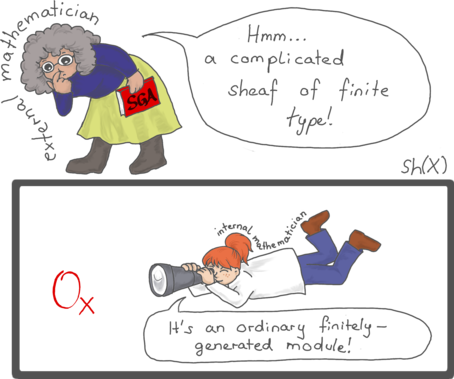
\includegraphics[width=0.7\textwidth]{external-internal-small}
    \par
  }

  \pause

  \small\centering
  \scalebox{0.83}{\begin{tabular}{ll}
    \toprule
    externally & internally to $\Sh(X)$ \\
    \midrule
    sheaf of sets & set \\
    %sheaf of rings & ring \\
    sheaf of modules & module \\
    sheaf of finite type & finitely generated module \\
    % finite locally free sheaf & finite free module \\
    % coherent sheaf & coherent module \\
    tensor product of sheaves & tensor product of modules \\
    % sheaf of Kähler differentials & module of Kähler differentials \\
    sheaf of rational functions & total quotient ring of~$\O_X$ \\
    dimension of $X$ & Krull dimension of~$\O_X$ \\
    spectrum of a sheaf of~$\O_X$-algebras & ordinary spectrum [with a twist] \\
    big Zariski topos of $X$ & big Zariski topos of the ring $\O_X$ [with a twist] \\
    higher direct images & sheaf cohomology \\
    \bottomrule
  \end{tabular}}

  \begin{columns}[c]
    \begin{column}{0.47\textwidth}
      \begin{exampleblock}{}
        \justifying
        Let $0 \to \F' \to \F \to \F'' \to 0$ be a short exact sequence
        of sheaves of~$\O_X$-modules. If~$\F'$ and~$\F''$ are of finite type,
        so is~$\F$.
      \end{exampleblock}
    \end{column}

    \begin{column}{0.1\textwidth}
      \vspace*{0.7em}
      \scalebox{3}{$\Leftarrow$}
    \end{column}

    \begin{column}{0.44\textwidth}
      \begin{exampleblock}{}
        \justifying
        Let~$0 \to M' \to M \to M'' \to 0$ be a short exact sequence of
        modules. If~$M'$ and~$M''$ are finitely generated, so is~$M$.
      \end{exampleblock}
    \end{column}
  \end{columns}
\end{frame}

\begin{frame}{Synthetic algebraic geometry}
  Usual approach to algebraic geometry: \hil{layer schemes above ordinary set theory}
  using either
  \begin{itemize}
    \item locally ringed spaces
    \small
    \begin{multline*}
      \text{set of prime ideals of~$\ZZ[X,Y,Z]/(X^n+Y^n-Z^n)$} + {} \\
      \text{Zariski topology} + \text{structure sheaf}
    \end{multline*}
    \normalsize
    \item or Grothendieck's functor-of-points account, where a scheme is a
    functor~$\Ring \to \Set$.
    \small\[ A \longmapsto \{ (x,y,z) \in A^3 \,|\, x^n+y^n-z^n=0 \} \]
  \end{itemize}
  \bigskip

  \jnote{1}{\footnotesize At the
  \fixedhref{https://sbseminar.wordpress.com/2009/08/06/algebraic-geometry-without-prime-ideals/}{Secret
  Blogging Seminar}, there was an insightful long-running discussion on the
  merits of the two approaches. Two disadvantages of the approach using
  locally ringed spaces is that the underlying topological spaces don't
  actually parametrize ``honest'', ``geometric'' points, but the more complex
  notion of irreducible closed subsets; and that they don't work well in a
  constructive setting. (For this, they would have to be replaced by locally
  ringed locales.)

  The functorial approach is more economical, philosophically rewarding, and
  works constructively. Given a functor~$F : \Ring \to \Set$, we imagine~$F(A)$
  to be the set of~``$A$-valued points'' of the hypothetical scheme described
  by~$F$, the set of ``points with coordinates in~$A$''. These sets have direct
  geometric meaning. However, typically only field-valued points are easy
  to describe. For instance, the functor representing projective~$n$-space is
  given on fields by
  \[ \begin{array}{r@{}c@{}l}
  K &{}\longmapsto{}& \text{the set of lines through the origin in~$K^{n+1}$} \\
  && \qquad \cong \{ [x_0 \hg \cdots \hg x_n] \,|\, \text{$x_i \neq 0$ for some~$i$} \},
  \end{array} \]
  whereas on general rings it is given by
  \[ \begin{array}{r@{}c@{}l}
    A &{}\longmapsto{}& \text{the set of quotients~$A^{n+1} \twoheadrightarrow P$,
    where~$P$ is projective,} \\
    && \qquad \text{modulo isomorphism}.
  \end{array} \]
  It is these more general kinds of points which impart a meaningful sense of
  cohesion on the field-valued points, so they can't simply be dropped from
  consideration.}

  \jnote{2}{This tension is resolved by observing that the category of
  functors~$\Ring \to \Set$ is a topos (the \emph{big Zariski topos} of~$\Spec(\ZZ)$)
  and that we can therefore employ its internal language. This language takes
  care of juggling stages behind the scenes. For instance, projective~$n$-space
  can be described by the naive expression
  \[ \{ (x_0,\ldots,x_n) : (\affl)^{n+1} \,|\, x_0 \neq 0 \vee \cdots \vee x_n
  \neq 0 \}/(\affl)^\times. \]
  This example illustrates our goal: to develop a synthetic account of
  algebraic geometry, in which schemes are plain sets and morphisms between
  schemes are maps between those sets. It turns out that there are many
  similarities with the well-developed synthetic account of differential
  geometry, but also important differences.}

  \pause

  \hil{Synthetic approach:} model schemes \hil{directly as sets} in
  the internal universe of the \mbox{\hil{big Zariski topos}} of a base scheme.
  \small
  \[ \{ (x,y,z) \? (\affl)^3 \,|\, x^n+y^n-z^n=0 \} \]
\end{frame}

\begin{frame}{The big Zariski topos}
  Let~$S$ be a fixed base scheme.
  \begin{varblock}{0.9\textwidth}{Definition}
    The \hil{big Zariski topos} $\Zar(S)$ of a scheme~$S$ is equivalently
    \begin{enumerate}
      \item the topos of sheaves over~$(\Aff/S)_{\mathrm{lofp}}$,
      \item the classifying topos of local rings over~$S$ or
      \item the classifying~$\Sh(S)$-topos of local~$\O_S$-algebras which are
      local over~$\O_S$.
    \end{enumerate}
  \end{varblock}

  \begin{itemize}
    \item For an~$S$-scheme~$X$, its functor of points $\ull{X} =
    \Hom_S(\cdot,X)$ is an object of~$\Zar(S)$. It feels like \hil{the set of
    points} of~$X$.
    \item In particular, there is the ring object~$\affl$ with~$\affl(T) =
    \O_T(T)$.
    \item This ring object is a \hil{field}: nonzero implies
    invertible. \\{} [Kock 1976]
  \end{itemize}

  \jnote{1}{The objects of the category~$(\Aff/S)_{\mathrm{lofp}}$ are
  morphisms of the form~$\Spec(R) \to S$ which are locally of finite
  presentation. (Other choices of resolving set-theoretical issues of size are
  also possible.)

  A functor~$F : (\Aff/S)_{\mathrm{lofp}}^\op \to \Set$ is a sheaf
  for the Zariski topology if and only if the diagram
  \[ F(T) \to
    \prod_i F(U_i) \rightrightarrows
    \prod_{j,k} F(U_j \cap U_k) \]
  is a limit diagram for any open covering~$T = \bigcup_i U_i$ of any
  scheme~$T \in (\Aff/S)_{\mathrm{lofp}}$.

  In the case that~$S = \Spec(A)$ is affine, the big Zariski topos of~$S$ is also
  simply called ``big Zariski topos of~$A$''. It is a subtopos of the topos of
  functors $\mathrm{Alg}(A) \to \Set$ and classifies local~$A$-algebras.

  From the internal point of view of~$\Sh(S)$, the sheaf~$\O_S$ of rings is
  just an ordinary ring, and one can construct internally to~$\Sh(S)$ the big
  Zariski topos of~$\O_S$. Externally, this construction will yield a certain
  bounded topos over~$\Sh(S)$. However, as indicated on the slide, this topos
  will \emph{not} coincide with the true big Zariski topos of~$S$. To
  construct the true big Zariski topos, one has to build, internally
  to~$\Sh(S)$, the classifying topos of local \emph{and local-over-$\O_S$}
  $\O_S$-algebras.}
\end{frame}

\begin{frame}{Synthetic constructions}
  \small
  $\hil{$\boldsymbol{\mathbb{A}^n}$} = (\affl)^n = \affl \times \cdots \times \affl$

  $\begin{array}{@{}r@{}c@{}l@{}}
    \hil{$\boldsymbol{\mathbb{P}^n}$} &\phantom{}=\phantom{}& \{ (x_0,\ldots,x_n) : (\affl)^{n+1} \,|\, x_0 \neq 0 \vee
    \cdots \vee x_n \neq 0 \}/(\affl)^\times \\
    &\cong& \text{set of one-dimensional subspaces of~$(\affl)^{n+1}$} \\
    &&\qquad \text{(with~$\O(-1) = (\ell)_{\ell \? \mathbb{P}^n}$, $\O(1) =
    (\ell^\vee)_{\ell \? \mathbb{P}^n}$)}
  \end{array}$

  $\hil{$\boldsymbol{\Spec(R)}$} = \Hom_{\mathrm{Alg}(\affl)}(R, \affl) =
    \text{set of $\affl$-valued points of $R$}$

  $\hil{$\boldsymbol{TX}$} = X^\Delta$, where $\Delta = \{ \varepsilon \? \affl \,|\, \varepsilon^2 = 0 \}$

  A subset $U \subseteq X$ is \hil{qc-open} if and only if for any $x : X$
  there exist $f_1,\ldots,f_n \? \affl$ such that $x \in U \Longleftrightarrow
  \exists i\_ f_i \neq 0$.

  A \hil{synthetic affine scheme} is a set which is in bijection
  with~$\Spec(R)$ for some synthetically quasicoherent~$\affl$-algebra~$R$.

  A \hil{finitely presented synthetic scheme} is a set which can be covered by
  finitely many qc-open f.p. synthetic affine schemes~$U_i$ such that the
  intersections~$U_i \cap U_j$ can be covered by finitely many qc-open f.p.
  synthetic affine schemes.

  \jnote{1}{In the internal universe of the big Zariski topos of a base
  scheme~$S$, $S$-schemes can simply be modeled by sets (enjoying the special
  property that, in a certain precise sense, they are locally affine). This
  slide expresses some of the basic constructions of~$S$-schemes in that
  language.

  Particularly nice are the following items.
  \begin{itemize}\justifying
    \item Projective~$n$-space can be given by the any of the two quite naive
    expressions displayed on the slide.
    \item Let~$X$ be an~$S$-scheme. We often think about a sheaves
    of~$\O_X$-modules over~$X$ by their fibers; but for a rigorous
    treatment in the standard foundations, we have to take the full sheaf
    structure into account; the fibers do not determine a sheaf
    uniquely.

    From the internal point of view of~$\Zar(S)$, a sheaf of~$\O_X$-modules is
    indeed simply a family of~$\affl$-modules, one~$\affl$-module for each
    element of~$\ull{X}$. The slide illustrates how we can define the Serre
    twisting sheaves in this language.
  \end{itemize}}

  \jnote{2}{\begin{itemize}\justifying
    \item The spectrum of an~$\affl$-algebra can be given by the naive
    expression displayed on the slide. It looks like this expression can't be
    right, ignoring any non-maximal ideals; however, it is.
    \item The big Zariski topos of an~$S$-scheme~$X$ is, from the internal
    point of view of~$\Zar(S)$, simply the slice topos~$\Set/\ull{X}$. Hence to
    give an~$X$-scheme simply amounts to giving an~$\ull{X}$-indexed family of
    sets.
  \end{itemize}

  Synthetic algebraic geometry has been developed up to the point of étale
  geometric morphisms. Much remains to be done: For instance, as of yet there
  is only an account of Čech methods for computing cohomology, there is not yet
  a synthetic treatment of true cohomology. Derived categories and intersection
  theory are also missing.}
\end{frame}

\begin{frame}{Relations between the Zariski toposes}
  The big Zariski topos is a topos over the small Zariski topos:
  \[ \begin{array}{crcl}
    \pi : & \Zar(A) &\longrightarrow& \Spec(A) \\
    & \text{local~$A$-algebra~$(A \xrightarrow{\alpha} B)$} &\longmapsto& (A \to A[(\alpha^{-1}[B^\times])^{-1}])
  \end{array} \]
  This morphism is \hil{connected} ($\pi^{-1}$ is fully faithful) and
  \hil{local}, so there is a preinverse
  \[ \begin{array}{rcl}
    \Spec(A) &\longrightarrow& \Zar(A) \\
    \text{local localization~$(A \to B)$} &\longmapsto& (A \to B)
  \end{array} \]
  which is a subtopos inclusion inducing an idempotent monad~$\sharp$ and an
  idempotent comonad~$\flat$ on~$\Zar(S)$.

  \begin{itemize}
  \justifying
    \item Internally to~$\Zar(S)$, $\Spec(S)$ can be constructed as the
    \hil{largest subtopos} where~$\flat \affl \to \affl$ is bijective.
    \item Internally to~$\Spec(S)$, $\Zar(S)$ can be constructed as the
    \hil{classifying topos} of local~$\O_S$-algebras which are local over~$\O_S$.
    \item $\Zar(A)$ is the \hil{lax pullback}~$(\Set
    \Rightarrow_{\Set[\Ring]} \Set[\LocRing])$.
  \end{itemize}

  \jnote{1}{Let~$A$ be a ring. By definition, we obtain a geometric
  morphism~$\Set \to \Set[\Ring]$ into the classifying topos of rings.
  There is also a geometric morphism~$\Set[\LocRing] \to \Set[\Ring]$, obtained
  by realizing that any local ring is in particular a ring. These morphisms fit
  together in a lax pullback square as follows:
  \[ \xymatrix{
    \Zar(A) \ar[r] \ar[d] & \Set[\LocRing] \ar[d] \\
    \Set \ar[r] \ar@{}[ur]^(.3){}="a"^(.7){}="b" \ar@{=>} "a";"b" & \Set[\Ring]
  } \]
  This observation is joint with Peter Arndt and Matthias Hutzler.

  Incidentally, the pseudo pullback of the morphism~$\Set[\LocRing] \to
  \Set[\Ring]$ along~$\Set \to \Set[\Ring]$ is not very interesting: It's the
  largest subtopos of~$\Set$ where~$A$ is a local ring. Assuming the law of
  excluded middle, this subtopos is either the trivial topos (if~$A$ is not
  local) or~$\Set$ (if~$A$ is local).

  There is also a way of realizing the little Zariski topos of~$A$ as a pseudo
  pullback, exploiting that the (localic) spectrum construction is geometric.
  See Section~12.6 of
  \fixedhref{https://rawgit.com/iblech/internal-methods/master/notes.pdf}{these
  notes} for details.
  }
\end{frame}


\section{The mystery of nongeometric sequents}

\begin{frame}{Properties of the affine line}
  \begin{itemize}
    \item $\affl$ is a local ring:
    \[ 1 \neq 0 \qquad\qquad \text{$x + y$ \inv} \Longrightarrow \text{$x$ \inv} \vee
    \text{$y$ \inv} \]
    \item $\affl$ is a field:
    \begin{align*}
      \neg(x = 0) &\Longleftrightarrow \text{$x$ invertible \quad [Kock 1976]} \\
      \neg(\text{$x$ invertible}) &\Longleftrightarrow \text{$x$ nilpotent}
    \end{align*}
    \item $\affl$ satisfies the axiom of microaffinity: Any map $f : \Delta \to
    \affl$ is of the form~$f(\varepsilon) = a + b \varepsilon$ for unique
    values~$a,b \? \affl$, where~$\Delta = \{ \varepsilon \? \affl \,|\,
    \varepsilon^2 = 0 \}$.
    \item Any map $\affl \to \affl$ is a polynomial.
    \item $\affl$ is anonymously algebraically closed: Any monic polynomial
    does \emph{not not} have a zero.
  \end{itemize}

  \jnote{1}{The axiom of microaffinity is a special instance of the
  \emph{Kock--Lawvere axiom} known from synthetic differential geometry. We'll
  see on the next slide that~$\affl$ validates an unusually strong form of the
  Kock--Lawvere axiom, not at all satisfied in the usual well-adapted models of
  synthetic differential geometry.

  The fact that, internally to~$\Zar(S)$, any map~$\affl \to \affl$ is a
  polynomial can be seen as a formal version of the general motto that in
  algebraic geometry, ``morphisms are polynomials''.}
\end{frame}

\begin{frame}{Synthetic quasicoherence}
  Recall~$\Spec(R) = \Hom_{\mathrm{Alg}(\affl)}(R, \affl)$ and consider the statement
  \[ \text{``the canonical map~$
    \begin{array}[t]{rcl}
      R &\longrightarrow& (\affl)^{\Spec(R)} \\
      f &\longmapsto& (\alpha \mapsto \alpha(f))
    \end{array}
  $ is bijective''}.
  \]
  \vspace*{-1em}

  \begin{itemize}
    \item True for~$R = \affl[X]/(X^2)$ (microaffinity).
    \item True for~$R = \affl[X]$ (every function is a polynomial).
    \item True for \hil{any} finitely presented~$\affl$-algebra~$R$.
  \end{itemize}

  Any known property of~$\affl$ follows from this \\
  \hil{synthetic quasicoherence}.

  \centering
  \begin{varblock}{0.6344\textwidth}{}
    \centering
    \hil{the mystery of nongeometric sequents}
    \par
  \end{varblock}

  \jnote{1}{Let~$R$ be an~$\affl$-algebra. An element~$f \in R$ induces
  an~$\affl$-valued function on~$\Spec(R)$; functions of this form can
  reasonably be called ``algebraic''. In a synthetic context, there should be
  no other~$\affl$-valued functions on~$\Spec(R)$ as these algebraic ones, and
  different algebraic expressions should yield different functions. This is
  precisely what the bijectivity of the displayed map expresses (in a positive
  way).

  In synthetic differential geometry, the closest cousin of synthetic algebraic
  geometry, the analogue of the displayed map is only bijective for Weil
  algebras such as~$\affl[X]/(X^2)$ or $\affl[X,Y]/(X^2,XY)$, not for arbitrary
  finitely presented~$\affl$-algebras. This is a major difference to synthetic
  differential geometry.}

  \jnote{2}{The notion of synthetic quasicoherence is interesting for a number
  of reasons:\vspace*{-1.2em}
  \begin{itemize}\justifying
    \item All currently known properties of~$\affl$, such as all the properties
    listed on the previous slide, follow from the statement that~$\affl$ is
    synthetically quasicoherent.

    For instance, here is how we can verify the field property. Let~$x \?
    \affl$ such that~$x \neq 0$. Set~$R = \affl/(x)$. Then~$\Spec(R) =
    \emptyset$. Thus~$(\affl)^{\Spec(R)}$ is a singleton. Hence~$R = 0$.
    Therefore~$x$ is invertible.
    \item Given an~$\affl$-module~$E$, we can formulate the following variant
    of the axiom of synthetic quasicoherence: ``For any finitely
    presented~$\affl$-algebra~$R$, the canonical map~$R \otimes_\affl E \to
    E^{\Spec(R)}$ is bijective.'' This axiom is satisfied if and only if~$E$ is
    induced by a quasicoherent sheaf of~$\O_S$-modules.
    \item The notion of synthetic quasicoherence is central to synthetic
    algebraic geometry. The notions of synthetic open immersions, closed
    immersion, schemes and several others all refer to synthetic
    quasicoherence.
  \end{itemize}}

  \jnote{3}{An anlogue of synthetic quasicoherence holds in the classifying
  topos of rings, demonstrating that even presheaf toposes can validate
  interesting nontrivial nongeometric sequents.

  We believe that an analogue of synthetic quasicoherence holds for the generic
  model of any geometric theory. This is work in progress. If true, this would
  yield a major source of nongeometric sequents in classifying toposes. Because
  of the many applications on nongeometric sequents, it's very desirable to
  possess such a source.

  The mystery of nongeometric sequents is this: On the one hand, they are very
  useful to have because of surprising applications; on the other hand, they
  are as of yet quite elusive.}
\end{frame}

{\usebackgroundtemplate{\begin{minipage}{\paperwidth}\vspace*{4.95cm}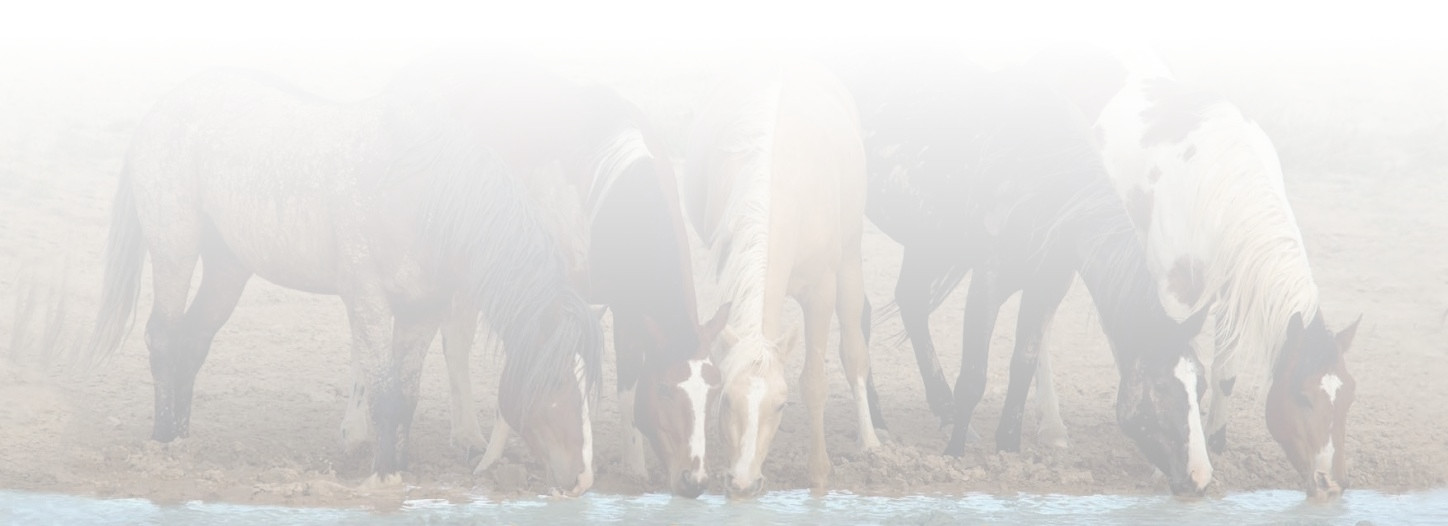
\includegraphics[width=\paperwidth]{topos-horses-lighter}\end{minipage}}
\begin{frame}{Classifying toposes in algebraic geometry}
  \small
  \centering
  \begin{tabular}{ll}
    \toprule
    (big) topos & classified theory \\\midrule
    Zariski & local rings [Hakim 1972] \\[0.6em]
    étale & separably closed local rings [Hakim 1972, Wraith 1979] \\[0.6em]
    \usebeamercolor[fg]{item}{fppf} & \usebeamercolor[fg]{item}{fppf-local rings} \\
    & \textcolor{red!90}{(conjecturally: algebraically closed local rings)} \\[0.6em]
    \textcolor{red!80}{ph} & \textcolor{red!80}{?? (conjecturally: algebraically closed valuation rings} \\
    & \qquad \textcolor{red!80}{validating the projective Nullstellensatz)} \\[0.6em]
    \usebeamercolor[fg]{item}{surjective} & \usebeamercolor[fg]{item}{algebraically closed geometric fields} \\[0.6em]
    \textcolor{red!80}{$\neg\neg$} & \textcolor{red!80}{?? (conjecturally: algebraically closed geometric} \\
    & \qquad \textcolor{red!80}{fields which are integral over the base)} \\[0.6em]
    \usebeamercolor[fg]{item}{infinitesimal} & \usebeamercolor[fg]{item}{local algebras together with a nilpotent ideal [Hutzler 2018]} \\[0.6em]
    \textcolor{red!100}{crystalline} & \textcolor{red!100}{??} \\
    \bottomrule
  \end{tabular}

  \jnote{1}{Toposes, and also more specifically classifying toposes, originated
  in algebraic geometry. It is therefore deeply embarassing that as of now,
  still very little is known about the theories classified by the major toposes
  in active use by algebraic geometers.
  \begin{center}
    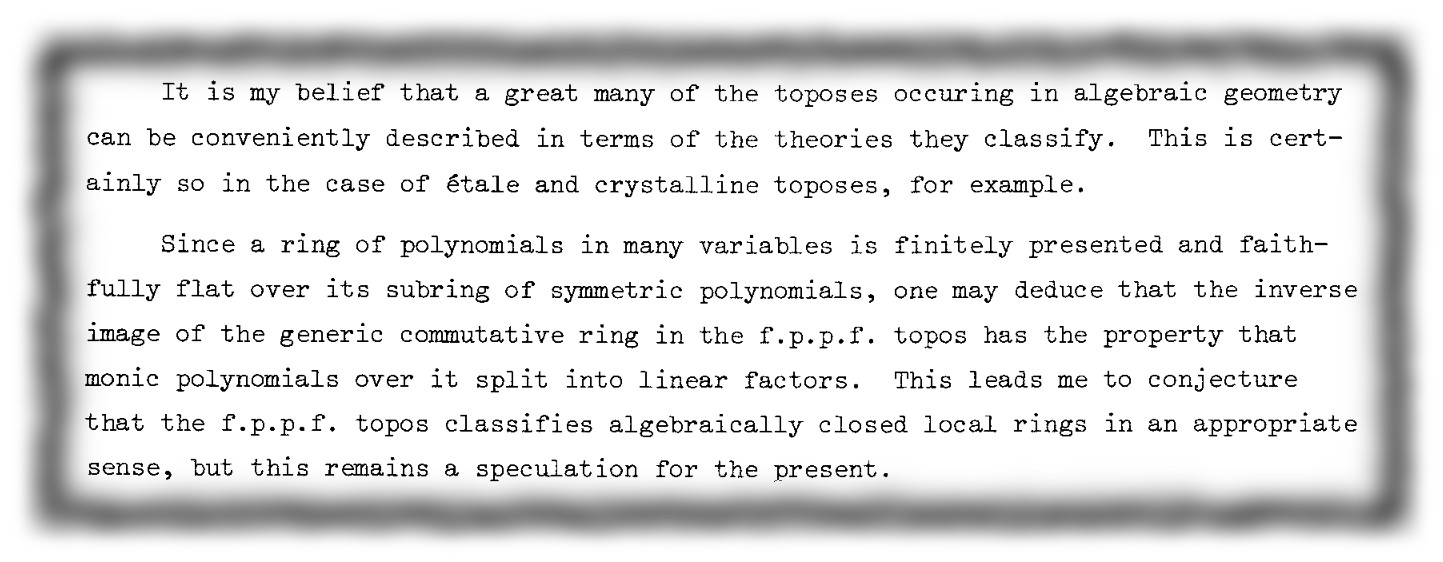
\includegraphics[width=0.99\textwidth]{wraith-generic-galois-theory} \\
    \footnotesize
    Gavin Wraith. Generic Galois theory of local rings. 1979.
  \end{center}}

  \jnote{2}{For almost forty years, only the big Zariski topos and its étale
  subtopos were understood in that way.
  \fixedhref{https://rawgit.com/iblech/internal-methods/master/notes.pdf}{These~2017
  notes} answer the question for the fppf topology and the surjective topology
  (in Section~21) and state conjectures for the ph topology and the
  double negation topology. However, while good to have, the answer for the
  fppf topology remains unsatisfactory, since Wraith's conjecture that the fppf
  topos classifies the simpler theory of algebraically closed local rings has
  neither been confirmed nor refuted.

  A couple of weeks ago, Matthias Hutzler managed to determine the theory
  classified by the big infinitesimal topos of a ring~$A$: It classifies
  pairs~$(B,\aaa)$ consisting of a local~$A$-algebra~$B$ and a nilpotent
  ideal~$\aaa \subseteq B$. Details will be in his forthcoming Master's thesis.
  He is currently working on answering the question for the closely related big
  crystalline topos.

  It will be exciting to learn what the crystalline topos and the many other
  toposes in algebraic geometry classify; how algebraic geometry can profit
  from these discoveries; and which new flavors of synthetic algebraic geometry
  they unlock.}
\end{frame}}

% XXX: Mehr Leute zitieren!
% XXX: Einordnung in Gesamtkontext (etwa SDG, Kock--Lawvere, Coquand & Co., ...)
% XXX: Folie zu klassifizierenden Topoi

\end{document}
